%  Typ dokumentu - článek, prezentace aj.
\documentclass[english]{article}

%  Nastaví vstupní a výstupní kódování znaků (encoding) a lokalizace
\usepackage[T1]{fontenc}
\usepackage[utf8]{inputenc}
\usepackage[english,czech]{babel}
\usepackage{icomma}

%  Formát papíru a odsazení od jeho okrajů
\usepackage[letterpaper]{geometry}
\geometry{verbose,tmargin=1.5cm,bmargin=2cm,lmargin=2cm,rmargin=2cm}

%  Umožňuje pracovat s grafikou
\usepackage{graphicx}
\usepackage{bigstrut}
\usepackage{epstopdf}

%  Automaticky odsadí i první paragraf v každé sekci
\usepackage{indentfirst}

%  Umožňuje rozdělovat obsah na více sloupců
\usepackage{multicol}
\usepackage{booktabs}
\usepackage{pgffor}

%  Umožňuje používat hypertextové odkazy, nastavuje jejich barvu a
%  vlastnosti
\usepackage[unicode]{hyperref}
\hypersetup{
colorlinks=true, citecolor=blue, filecolor=blue, linkcolor=blue,
urlcolor=blue
}

%  Umožnění odstranění italiky u jednotek
\newcommand{\unit}[1]{\mathrm{#1}}

%  Formátování stránek, empty = odstraní číslování
% \pagestyle{empty}

%  Řádkování
\linespread{1.2}

%  Lepší zobrazování matematiky (rozšíření sum o \limits atd.)
\everymath{\displaystyle}
\usepackage{amsmath, amsthm, amssymb}

% Umožní psát přes \mathbb{N/R/Q/..} množiny čísel
\usepackage{amssymb}

%  Velikost fontu matematických výrazů v dokumentu lze pro danou
% základního fontu dokumentu upravit pomocí:
% \DeclareMathSizes{X}{Y}{Z}{U} kde:
% X je velikost fontu v dokumentu, pro kterou se matematika upraví
% Y je standartní velikost fontu matematiky
% Z je velikost fontu zmenšených (vnořených výrazů)
% U je velikost fontu ještě více zmenšených (vnořených výrazů).
\DeclareMathSizes{10}{10.5}{9}{9}

%  Nastaví autora, název, datum, skupinu měření apod. (můj vlastní
% příkaz, umožní znovu-použití v dokumentu)
\newcommand{\Author}{David Roesel}
\newcommand{\Coauthor}{Tereza Schönfeldová}
\newcommand{\Institute}{FJFI ČVUT v Praze}
\newcommand{\Subject}{FYZIKÁLNÍ PRAKTIKUM II}
\newcommand{\Group}{7}
\newcommand{\Circle}{ZS 7}
\newcommand{\Title}{Úloha \#11  \\Termické emise elektronů}
\newcommand{\Date}{24.3.2014}

% Začátek dokumentu - Formátování na výstup
\begin{document}

% Interní proměnné, možno zobrazovat u prezentací, používají se při
% generování pomocí \titlepage apod.
\author{\Author}
\title{\Title}
\date{\Date}

%  Lokalizace některých názvů do češtiny
\renewcommand{\figurename}{Obr.}
\renewcommand{\tablename}{Tab.}
\renewcommand{\refname}{Reference}

% --- Hlavička dokumentu -----------------------------------------------

\setlength{\parindent}{0cm}
\begin{multicols}{2}
\textbf{\Subject \\
        \Institute \\[0.1cm]
%\large  \Title \\[0.5cm]
\Title \\[0.5cm]
}
\begin{tabular}{rlrl}
\large Datum měření: & \Date & \large Skupina: & \Group \\
\large Jméno: & \Author & \large Kroužek:  & \Circle\\
\large Spolupracovala: & \Coauthor &\large Klasifikace:\\
\end{tabular}

\begin{flushright}

\includegraphics[scale=0.28]{../../_meta/fjfi_standart.pdf}
\hspace{0.2cm}

\includegraphics[scale=0.28]{../../_meta/cvut_standart.pdf}
\end{flushright}
\end{multicols}
\hrule
\vspace{0.5cm}

% ----------------------------------------------------------------------


% --- Tělo dokumentu ---------------------------------------------------
\setlength{\parindent}{0.5cm}
\section{Pracovní úkoly}
% #rost
\begin{enumerate}
  \item Změřte závislost emisního proudu katody na kladném anodovém napětí
    v rozmezí (100 -- 600) V, po cca 100~V, při konstantní teplotě katody.
    Měření proveďte pro 6 -- 10 teplot v rozmezí 1800 až 2500 K. Teplotu
    měřte pyrometrem.
  \item Výsledky měření podle bodu 1 vyneste do grafu (viz. Obr. 4
    v zadání úlohy \cite{bib:zadani} - vyneste závislost $\ln(I)$ na~$\sqrt{U}$),
    určete hodnoty emisního proudu $I_0$ a nakreslete Richardsonovu přímku.
  \item Vypočtěte výstupní práci $\varphi_v$ a určete hodnotu Richardsonovy
    konstanty $A$, v obou případech zkuste odhadnout chybu. Diskutujte 
    rozdíl oproti očekávané hodnotě.
  \item Změřte závislost náběhového proudu $I_a=f(U_{KA})$ pro deset 
    hodnot záporného anodového napětí $U_{KA}$ při konstantním žhavícím
    proudu $I_{\check{z}h}$. Měřte v rozsahu -10 až 0 V, 1700 -- 2100 K.
  \item Měření podle bodu 4. proveďte pro šest různých hodnot žhavícího 
    proudu $I_{\check{z}h}$. Pro každou hodnotu žhavícího proudu změřte teplotu 
    středu katody radiačním pyrometrem.
  \item Průběh $I_a=f(U_{KA})$ vyneste do grafu (viz. Obr. 3 v zadaní
    úlohy \cite{bib:zadani}, vyneste závislost ln$I$ na $U$). Z průběhů
    náběhového proudu pomocí vzorce (\ref{eq:fit_nabeh}) odhadněte 
    příslušné teploty katody a porovnejte je s teplotami změřenými pyrometrem.
  \item Spolu s každým měřením teploty v předchozích úlohách si poznamenejte
    i napětí a proud na žhavícím zdroji. Na základě Stefan-Boltzmanova zákona
    (\ref{eq:stefan}) a ve vláknu disipovaného výkonu $P=U_{\check{z}h}I_{\check{z}h}$ 
    odhadněte teplotu vlákna, porovnejte s hodnotou změřenou pyrometrem. 
    Vyneste do grafu a rozdíl diskutujte.
\end{enumerate}

\section{Vypracování}

	\subsection{Použité přístroje}
		Speciální dioda s wolframovou žhavnou katodou trvale čerpaná vakuovým systémem, regulovatelný zdroj 20 V, žhavicí transformátor, regulovatelný zdroj 60 V, voltmetr, ampérmetr, miliampérmetr, nanoampérmetr, regulační transformátor 0 -- 220 V.
			
	\subsection{Teoretický úvod}
		Dobrou představou, která stačí pro popsání většiny jevů vyskytujících se v kovu, je model krystalické mřížky složené z kladných iontů a záporných elektronů, které se mezi nimi pohybují. V závislosti na teplotě kovu mají tyto elektrony jistou kinetickou energii. Energii potřebnou k opuštění látky nazýváme výstupní prací $\varphi_v$. Výstupní rychlost se řídí Maxwell-Boltzmannovým rozdělením. Poté, co elektrony opustí látku, vytvoří oblak prostorového náboje, který potlačuje další emisi elektronů. 
		
		Mějme dvě destičky z kovu (katodu a anodu ve vzdálenosti $a$) a nechť je mezi nimi nulový nebo malý záporný potenciálový rozdíl $\varphi_a$. Pak můžeme pro koncentraci elektronů $n_x$ v nějaké vzdálenosti $x$ od katody napsat vztah
		\begin{equation}
			n_x = n_0\cdot\mathrm{exp}\left(\frac{e\varphi_x}{kT}\right),
		\end{equation} 
		kde $n_0$ je koncentrace elektronů u katody, $k = 1,38\cdot10^{-23}~\mathrm{W\cdot s \cdot K^{-1}}$ Boltzmannova konstanta, $e=1,602\cdot10^{-19}$~C velikost náboje elektronu a $T$ termodynamická teplota. Z toho potom platí pro celkový proud $I_a$ vztah
		\begin{equation}
			I_a = I_0\cdot\mathrm{exp}\left(\frac{e\varphi_a}{kT}\right),
		\end{equation}
		kde $I_0$ představuje ideální nasycený proud diodou. Pokud tento vztah zlogaritmujeme, dostaneme
		\begin{equation}
			\mathrm{ln}I_a = \mathrm{ln}I_0+\frac{e}{kT}\varphi_a \qquad
			\Leftrightarrow \qquad y=a+bx,
			\label{eq:fit_nabeh}
		\end{equation}
		z čehož plyne, že ze směrnice naměřené závislosti $I_a(\varphi_a)$ můžeme určit teplotu katody. To provedeme pomocí lineárního proložení, kde $a=\mathrm{ln}I_0$ a $b=\frac{e}{kT}$, čímž pádem budeme moci spočítat teplotu katody $T$ podle vztahu
		\begin{equation}
			T=\frac{e}{kb}.
			\label{eq:teplota_nabeh}
		\end{equation}
		
		Zajímají-li nás možné zdroje chyb, měli bychom se věnovat následujícím oblastem:
		\begin{itemize}
			\item vliv prostorového náboje (je vhodné měřené proudy udržovat co nejmenší)
			\item vliv elektronů vyražených krátkovlnným zářením z katody
			\item vliv sekundárních elektronů vyražených z katody
		\end{itemize}
		
		Chceme-li určit výstupní práci elektronu $e\varphi_v$, můžeme tak učinit (za předpokladu, že je dioda z námi studovaného kovu) měřením tzv. \emph{nasyceného proudu}. Vliv prostorového náboje zmenšíme tím, že budeme volit polaritu potenciálového rozdílu mezi anodou a katodou tak, aby elektrické pole urychlovalo elektrony směrem k anodě. Jakmile napětí $U_{KA}$ přesáhne nějakou úroveň, proud diodou $I_a$ prakticky neroste a můžeme ho označit za nasycený. Jeho hodnotu zvládneme určit ve shodě se Schottkyho teorií, ze které jde odvodit, že 
		\begin{equation}
			\mathrm{ln}I_a = \mathrm{ln}I_0+K\cdot\sqrt{\varphi_a}
			\qquad\Leftrightarrow\qquad y=a+bx,
			\label{eq:sqrt_fit}
		\end{equation}
		kde $I_a$ je procházející proud, $I_0$ proud nasycený, $K$ konstanta závislá na teplotě a velikosti měřící anody a katody a $\varphi_a$ napětí na anodě.
		
		Pro nasycený proud $I_0$ dále platí:
		\begin{equation}
			I_0 = SAT^2\mathrm{exp}\left(-\frac{e\varphi_v}{kT}\right),
		\end{equation}
		kde $S$ je povrch katody, $A$ tzv. \emph{Richardsonova konstanta}, $T$ termodynamická teplota, $\varphi_v$ výstupní potenciál (z něj spočítaná výstupní práce pro elektron $e\varphi_v$). Hodnota Richardsonovy konstanty se pro wolfram typicky pohybuje kolem $80\cdot 10^4~A\cdot m^{-2} \cdot K^{-2}$ \cite{bib:tabulky}. Tento vztah můžeme také zlogaritmovat a dostáváme
		\begin{equation}
			\mathrm{ln}I_0-2\mathrm{ln}T=\mathrm{ln}SA-\frac{e\varphi_v}{k}\frac{1}{T}
			\qquad\Leftrightarrow\qquad y=a-bx,
			\label{eq:fit_richardson}
		\end{equation}
		tedy značíme $y=\mathrm{ln}I_0-2\mathrm{ln}T$, $a=\mathrm{ln}SA$, $b=\frac{e\varphi_v}{k}$ a $x=\frac{1}{T}$. Rovnici $y=a-bx$ nazýváme \emph{Richardsonovou přímkou}. Z koeficientu $b$ můžeme určit výstupní práci a Richardsonovu konstantu podle 
		\begin{equation}
			\varphi_v = \frac{bk}{e}, \qquad A=\frac{e^a}{S},
			\label{eq:phi_a_A}
		\end{equation}
		kde zachováváme předchozí značení.
		
		Během celé úlohy budeme určovat teplotu spektrálním pyrometrem, který změří intenzity (ve formě napětí) červeného a modrého světla $E_{\check{c}}$ a $E_m$, a my tak můžeme určit teplotu pozorovaného objektu podle vztahu
		\begin{equation}
			\mathrm{log_{10}}\left(\frac{E_{\check{c}}}{E_m}\right) = c_1+\frac{c_2}{T},\qquad kde~c_1 = -0,2457~a~c_2 = 2146,35.
			\label{eq:pyro}
		\end{equation}
		
		Zároveň budeme měřit teplotu vlákna pomocí Stefan-Boltzmannova zákona pro vyzařování černého tělesa, který má tvar 
		\begin{equation}
			P = U_{\check{z}h}I_{\check{z}h} = S\sigma T^4 \qquad \Rightarrow \qquad T=\left(\frac{U_{\check{z}h}I_{\check{z}h}}{S\sigma}\right)^\frac{1}{4},
			\label{eq:stefan}
		\end{equation}
		kde $\sigma=5,67\cdot10^{-8}~\mathrm{W\cdot m^{-2}\cdot K^{-4}}$ je tzv. \emph{Stefan-Boltzmannova konstanta}.
		
	\subsection{Postup měření}
		Vzhledem k poškození aparatury předchozí skupinou jsme měření neprováděli sami, ale obdrželi jsme všechna naměřená data od asistentů. Postup jsme si tak nemohli vyzkoušet a nejsme schopni diskutovat jeho výhody a úskalí. V případě, že bychom úlohu měřili, postupovali bychom podle postupu uvedeného v následujících odstavcích.
		
		\subsubsection{Měření nasyceného proudu}
			Obvod zapojíme podle nákresu na Obr. \ref{fig:s_aparatura_nasyc} a po sestavení zapneme vývěvy. Po dosažení jistého stupně vakua započneme měření proudu $I_a$ v závislosti na anodovém napětí $U_a$ za držení konstantní teploty. Používáme přitom zdroj proměnného kladného napětí 0-600 V a anodový proud měříme ve většině případů miliampérmetrem. Před každým měřením nejprve nastavíme konkrétní žhavicí proud $I_{\check{z}h}$ a napětí $U_{\check{z}h}$ a tyto zaznamenáme. K tomu navíc změříme pyrometrem intenzity (potažmo napětí) odpovídající modré $U_m$ a červené $U_{\check{c}}$ barvě a jejich hodnoty si zapíšeme. Z těchto zapsaných hodnot budeme schopni dvěma způsoby určit teplotu katody.   
			
		\subsubsection{Měření náběhového proudu}
			Toto měření provádíme takřka stejně jako měření minulé, až na to, že používáme generátor záporného napětí (budeme tedy adekvátně tomu vynášet závislost přímo na $U_a$ a ne na jeho odmocnině) a proudy měříme mikroampérmetrem.
			
			
			Při měření termoemise je klíčové, aby měl povrch katody všude stejnou teplotu, čehož dosahujeme zapojením znázorněným na Obr. \ref{fig:s_dida}. Měřící anoda je obklopena dvěma dalšími pomocnými anodami, které brání odvodu tepla do přívodu žhavicího proudu.
							
\clearpage
	\subsection{Naměřené hodnoty}
		Výpočty jsme prováděli z dodaných hodnot. Plochu katody jsme určili z poloměru $r=0,1$~mm a délky $d=2$~cm na $S=1,26\cdot10^{-5}~\mathrm{m}^2$. Konstanty $k$ a $e$ použité ve výpočtech jsou číselně uvedeny v teoretickém úvodu.
		
		Pro všechna měření jsme vypočítali teplotu vlákna pomocí Stefan-Boltzmannova zákona (\ref{eq:stefan}) a její hodnoty jsme vynesli do grafu na Obr. \ref{fig:g_stefpyro} v závislosti na teplotě změřené pyrometrem.
		
		\subsubsection{Měření nasyceného proudu}
			Naměřené a vypočítané hodnoty jsou uvedeny v Tab. \ref{tab:nasyc}. Výsledky měření prvního úkolu jsou jako závislost ln$I$ na $\sqrt{U}$ vyneseny v grafu na Obr. \ref{fig:g_termise}. Richardsonova přímka odpovídající parametrům fitů je vynesena v grafu na Obr. \ref{fig:g_termiserich}. Z ní jsme určili výstupní práci elektronu a Richardsonovu konstantu jako
			\begin{equation}
				e\varphi_v = e(4,3\pm0,3)~\mathrm{eV}, \qquad A = 127462~\mathrm{A\cdot m^{-2}\cdot K^{-2}}.
			\end{equation} 
			
% Table generated by Excel2LaTeX from sheet 'emisny prud'
\begin{table}[htbp]
  \centering
% Table generated by Excel2LaTeX from sheet 'emisny prud'
\begin{tabular}{|r|r|r|r|r|r|r|}
\hline
\boldmath{}\textbf{$I_{\check{z}h}$ [A]}\unboldmath{} & 3,3   & 3,0     & 2,8   & 2,6   & 3,1   & 2,9 \bigstrut\\
\hline
\boldmath{}\textbf{$U_{\check{z}h}$ [V]}\unboldmath{} & 6,9   & 6,2   & 5,4   & 4,9   & 6,5   & 5,9 \bigstrut\\
\hline
\boldmath{}\textbf{$T_{stef}$ [K]}\unboldmath{} & 2380  & 2260  & 2150  & 2060  & 2310  & 2210 \bigstrut\\
\hline
\boldmath{}\textbf{$\sigma_{T_{stef}}$ [K]}\unboldmath{} & 20    & 20    & 20    & 20    & 20    & 20 \bigstrut\\
\hline
\boldmath{}\textbf{$U_{\check{c}}$ [mV]}\unboldmath{} & 163,42 & 147,07 & 129,51 & 115,42 & 149,36 & 135,61 \bigstrut\\
\hline
\boldmath{}\textbf{$U_{m}$ [mV]}\unboldmath{} & 31,05 & 24,04 & 17,59 & 13,82 & 26,94 & 21,28 \bigstrut\\
\hline
\boldmath{}\textbf{$T_{pyro}$ [K]}\unboldmath{} & 2219,7 & 2079,2 & 1928,9 & 1838,5 & 2169,0 & 2044,1 \bigstrut\\
\hline
\boldmath{}\textbf{$\sigma_{T_{pyro}}$ [K]}\unboldmath{} & 0,3   & 0,4   & 0,4   & 0,5   & 0,4   & 0,4 \bigstrut\\
\hline
\boldmath{}\textbf{$U_{KA}$ [V]}\unboldmath{} & \boldmath{}\textbf{$I_{a-U_1}$ [mA]}\unboldmath{} & \boldmath{}\textbf{$I_{a-U_2}$ [mA]}\unboldmath{} & \boldmath{}\textbf{$I_{a-U_3}$ [mA]}\unboldmath{} & \boldmath{}\textbf{$I_{a-U_4}$ [mA]}\unboldmath{} & \boldmath{}\textbf{$I_{a-U_5}$ [mA]}\unboldmath{} & \boldmath{}\textbf{$I_{a-U_6}$ [mA]}\unboldmath{} \bigstrut\\
\hline
100   & 1,930 & 0,280 & 0,046 & 0,009 & 0,710 & 0,133 \bigstrut\\
\hline
200   & 2,040 & 0,310 & 0,048 & 0,009 & 0,760 & 0,140 \bigstrut\\
\hline
300   & 2,080 & 0,325 & 0,050 & 0,010 & 0,790 & 0,148 \bigstrut\\
\hline
400   & 2,180 & 0,335 & 0,052 & 0,010 & 0,810 & 0,153 \bigstrut\\
\hline
500   & 2,260 & 0,345 & 0,053 & 0,010 & 0,840 & 0,155 \bigstrut\\
\hline
550   & 2,320 & 0,350 & 0,054 & 0,010 & 0,860 & 0,158 \bigstrut\\
\hline
\boldmath{}\textbf{$I_{0-U_i}$ [mA]}\unboldmath{} & 1,680 & 0,243 & 0,041 & 0,008 & 0,623 & 0,117 \bigstrut\\
\hline
\boldmath{}\textbf{$\sigma_{I_{0-U_i}}$ [mA]}\unboldmath{} & 0,030 & 0,006 & 0,001 & 0,001 & 0,007 & 0,002 \bigstrut\\
\hline
\end{tabular}%

    \caption
    {
    Naměřené a vypočítané hodnoty pro měření nasyceného proudu;
    $I_{\check{z}h}$ a $U_{\check{z}h}$ jsou žhavící proud a napětí změřené s chybou $0,1$~A a $0,1$~V, 
    $T_{stef}$ a $\sigma_{T_{stef}}$ teplota určená Stefan-Boltzmannovým zákonem (\ref{eq:stefan}) se svou chybou (\ref{eq:chyba_neprime_mereni}), 
    $U_{\check{c}}$ a $U_{m}$ napětí změřené pyrometrem s chybou $0,01$~mV a
    $T_{pyro}$ a $\sigma_{T_{pyro}}$ teplota určená z tohoto napětí dle (\ref{eq:pyro}) i s chybou (\ref{eq:chyba_neprime_mereni}). $U_{KA}$ je napětí mezi katodou a anodou, $I_{a-U_i}$ celkový proud pro každé měření a $I_{0-U_i}$, $\sigma_{I_{0-U_i}}$  hodnota nasyceného proudu získaná i s chybou z fitu (\ref{eq:sqrt_fit}).
    }
    
      
  \label{tab:nasyc}%
\end{table}%
\clearpage
		\subsubsection{Měření náběhového proudu}
			Naměřené a vypočítané hodnoty jsou uvedeny v Tab. \ref{tab:nabeh}. Průběh $I_a=f(U_a)$ je vynesen do grafu na Obr. \ref{fig:g_nabeh}. Pomocí vzorce (\ref{eq:teplota_nabeh}) jsme z něj odhadli teploty $T_1$, $T_2$ katody na 
			\begin{equation}
				T_1 = (8100\pm200)~\mathrm{K}, \qquad T_2 = (11200\pm300)~\mathrm{K}.
			\end{equation}
			
% Table generated by Excel2LaTeX from sheet 'nabehovy prud'
\begin{table}[htbp]
\catcode`\-=12 % HAX na enable cline v českym bable
  \centering
   % Table generated by Excel2LaTeX from sheet 'nabehovy prud'
    \begin{tabular}{|r|r|r|r|r|}
    \hline
    \boldmath{}\textbf{$I_{\check{z}h}\pm\sigma_{I_{\check{z}h}}$ [A]}\unboldmath{} & 4,1   & 0,1   & 3,6   & 0,1 \bigstrut\\
    \hline
    \boldmath{}\textbf{$U_{\check{z}h}\pm\sigma{U_{\check{z}h}}$ [V]}\unboldmath{} & 9,9   & 0,1   & 8,2   & 0,1 \bigstrut\\
    \hline
    \boldmath{}\textbf{$T_{stef}\pm\sigma_{T_{stef}}$ [K]}\unboldmath{} & 2750  & 20    & 2540  & 20 \bigstrut\\
    \hline
    \boldmath{}\textbf{$U_{\check{c}}\pm\sigma_{U_{\check{c}}}$ [mV]}\unboldmath{} & 180,23 & 0,01  & 162,54 & 0,01 \bigstrut\\
    \hline
    \boldmath{}\textbf{$U_{m}\pm\sigma_{U_{m}}$ [mV]}\unboldmath{} & 40,71 & 0,01  & 26,87 & 0,01 \bigstrut\\
    \hline
    \boldmath{}\textbf{$T_{pyro}\pm\sigma_{T_{pyro}}$ [K]}\unboldmath{} & 2406,7 & 0,3   & 2089,1 & 0,3 \bigstrut\\
    \hline
    \multicolumn{1}{r|}{} & \boldmath{}\textbf{$U_{a1}~\mathrm{[V]}$ }\unboldmath{} & \boldmath{}\textbf{$I_{a1}~\mathrm{[\mu A]}$  }\unboldmath{} & \boldmath{}\textbf{$U_{a2}~\mathrm{[V]}$ }\unboldmath{} & \boldmath{}\textbf{$I_{a2}~\mathrm{[\mu A]}$  }\unboldmath{} \bigstrut\\
    \cline{2-5}\multicolumn{1}{r|}{} & -3,8  & 4,2   & -3,5  & 82,0 \bigstrut\\
    \cline{2-5}\multicolumn{1}{r|}{} & -4,0  & 3,6   & -4,0  & 55,0 \bigstrut\\
    \cline{2-5}\multicolumn{1}{r|}{} & -4,2  & 2,8   & -4,5  & 36,0 \bigstrut\\
    \cline{2-5}\multicolumn{1}{r|}{} & -4,4  & 2,0   & -5,0  & 23,0 \bigstrut\\
    \cline{2-5}\multicolumn{1}{r|}{} & -4,6  & 1,7   & -5,5  & 13,0 \bigstrut\\
    \cline{2-5}\multicolumn{1}{r|}{} & -4,8  & 1,2   & -6,0  & 8,0 \bigstrut\\
    \cline{2-5}\multicolumn{1}{r|}{} & -5,0  & 0,8   & -6,5  & 4,0 \bigstrut\\
    \cline{2-5}\multicolumn{1}{r|}{} & -5,2  & 0,6   & -7,0  & 2,0 \bigstrut\\
    \cline{2-5}\multicolumn{1}{r|}{} & -5,4  & 0,5   & -7,5  & 1,5 \bigstrut\\
    \cline{2-5}\multicolumn{1}{r|}{} & -5,6  & 0,3   & -8,0  & 1,0 \bigstrut\\
    \cline{2-5}\multicolumn{1}{r|}{} & -5,8  & 0,3   & \multicolumn{1}{r}{} & \multicolumn{1}{r}{} \bigstrut\\
    \cline{2-3}\end{tabular}%
    
  \caption{
Naměřené a vypočítané hodnoty pro měření náběhového proudu;
    $I_{\check{z}h}$ a $U_{\check{z}h}$ jsou žhavící proud a napětí,
    $T_{stef}$ a $\sigma_{T_{stef}}$ teplota určená Stefan-Boltzmannovým zákonem (\ref{eq:stefan}) se svou chybou (\ref{eq:chyba_neprime_mereni}), 
    $U_{\check{c}}$ a $U_{m}$ napětí změřené pyrometrem a
    $T_{pyro}$ a $\sigma_{T_{pyro}}$ teplota určená z tohoto napětí dle (\ref{eq:pyro}) i s chybou (\ref{eq:chyba_neprime_mereni}). $U_{a(1/2)}$ je napětí mezi katodou a anodou, $I_{a(1/2)}$ celkový proud pro každé měření.	
  }
  \label{tab:nabeh}%
\end{table}%
 						
	\subsection{Diskuse}
		Vzhledem k tomu, že jsme žádné z hodnot neměřili my, nebudeme se v diskusi věnovat možnému zpřesnění výsledků změnou postupu měření. Taktéž můžeme jen těžko soudit, jak moc se dá věřit chybovým intervalům určeným přístrojem a kde se pohybuje reálná chyba naměřených hodnot. 
		
		Můžeme se však rozhodně vyjádřit k vypočítané Richardsonově konstantě $A$, u které jsme v naměřených hodnotách ani neuváděli chybu, vzhledem k tomu, že vyšla větší než $150\%$. Velikost této chyby byla způsobena velkou relativní chybou parametru $a=(0,5\pm1,5)$, ze kterého se $A$ přímo počítá. Hodnota se však řádově shoduje s teoretickou $A=80\cdot 10^4~A\cdot m^{-2} \cdot K^{-2}$. Nemůžeme říci, že by se nám ji podařilo změřit, ale náš výsledek zároveň není při uvažování chybového intervalu v rozporu s teoretickým předpokladem. Výsledná hodnota výstupního potenciálu elektronu $\varphi_v = (4,3\pm0,3)~\mathrm{V}$ je již mnohem blíže předpokládané hodnotě $4,5$ V a můžeme říci, že se nám ji podařilo úspěšně určit.
		
		Místo šesti zadaných měření náběhového proudu jsme obdrželi data z pouze dvou. Odhady teploty katody získané z proložení těchto hodnot jsou však zcela nesmyslné. Jako příklad uveďme první (a méně odlišnou) z nich, která nám vyšla $T_1 = (8100\pm200)~\mathrm{K}$, což absolutně neodpovídá hodnotě změřené pyrometrem $(2406,7\pm0,3)$~K. Tato nesrovnalost je buď zapříčiněna nedokonalostí experimentu, malým množstvím naměřených a tím pádem proložených hodnot, nebo tím, že námi použité teoretické vztahy neodpovídají sestavení pokusu.
		
		Měření teploty pomocí Stefan-Boltzmannova zákona (\ref{eq:stefan}) dává podle grafu na Obr. \ref{fig:g_stefpyro} značně odlišné hodnoty od měření spektrálním pyrometrem. Vzhledem k tomu, že bereme pro její výpočet absolutně přesné rozměry wolframového vlákna, bude reálná chyba pomocí ní spočítaných hodnot klidně i o řád vyšší. Za nejpřesněji určenou hodnotu teploty bereme tedy (i s přihlédnutím k velikosti její chyby) tu, která byla změřena spektrálním pyrometrem. Jedna z hodnot je v grafu zcela evidentně mimo předpokládanou (byť posunutou) lineární závislost $y=ax$ - čekali bychom ji ve stejné vertikální poloze více vpravo (tak jako první hodnotu z měření náběhového proudu). Vzhledem k tomu, že jsme data neměřili, můžeme těžko odhadnout, čím byla chyba způsobena.
	
\section{Závěr}
	Zpracovali jsme data změřené závislosti emisního proudu katody na kladném anodovém napětí v rozmezí (100--600)~V při konstantní teplotě katody, která byla měřena pyrometrem. Výsledky tohoto měření jsme vynesli do grafu, pro každé z nich jsme určili hodnoty emisního proudu $I_0$ a nakreslili jsme Richardsonovu přímku. Úspěšně jsme určili výstupní práci $e\varphi_v$ a méně úspěšně jsme se pak o to samé pokusili u Richardsonovy konstanty $A$. V obou případech jsme spočítali a diskutovali chyby.   
	
	Zpracovali jsme data změřené závislosti náběhového proudu $I_a = f(U_{KA})$ při konstantním žhavícím proudu $I_{\check{z}h}$. Měření bylo provedeno pro dvě různé hodnoty tohoto žhavícího proudu a hodnoty obou měření jsme vynesli do grafu. Z průběhů náběhového napětí jsme odhadli příslušné teploty katody a diskutovali jsme jejich nesrovnalosti s teplotami změřenými pyrometrem. 
	
	U každého úkolu jsme z proudu a napětí na žhavícím zdroji vypočítali teplotu vlákna pomocí Stefan - Boltzmannova zákona a vypočítané hodnoty jsme porovnali s hodnotami změřenými pyrometrem. Výsledky jsme vynesli do grafu a diskutovali.

\section {Použitá literatura}
% --- Literatura a reference -------------------------------------------
\begingroup
\renewcommand{\section}[2]{}

\begin{thebibliography}{9}
\bibitem{bib:zadani} Kolektiv KF, \emph{Návod k úloze: Termické emise elektronů} [Online], [cit. \today] \newline http://praktikum.fjfi.cvut.cz/pluginfile.php/424/mod\_resource/content/7/termo\_2013\_05.pdf

\bibitem{bib:zadani2} Kolektiv KF, \emph{Doplněk návodu k úloze: Spektrální pyrometr} [Online], [cit. \today] \newline http://praktikum.fjfi.cvut.cz/pluginfile.php/1624/mod\_resource/content/5/pyromet\_navod.pdf

%\bibitem{bib:h3} Petr Chaloupka, \emph{Jak zpracovávat data} [Online], [cit. \today] \newline  https://dl.dropboxusercontent.com/u/11296940/zfm/h3.pdf

%\bibitem{bib:navody} Kolektiv KF, \emph{Návody k přístrojům} [Online], [cit. \today] \newline http://praktikum.fjfi.cvut.cz/documents/chybynav/navody-o.pdf

\bibitem{bib:chyby} Kolektiv KF, \emph{Chyby měření} [Online], [cit. \today] \newline http://praktikum.fjfi.cvut.cz/documents/chybynav/chyby-o.pdf

%\bibitem{bib:ctverce} Kolektiv KACH UPOL, \emph{Hodnocení analytických výsledků} [Online], [cit. \today] \newline http://ach.upol.cz/ucebnice/hodnoceni7.htm

\bibitem{bib:tabulky} J. Mikulčák a kol., Matematické, fyzikální a chemické tabulky \& vzorce. Prometheus,
Praha 2009.\newline
ISBN 978-80-7196-264-9

%\bibitem{bib:repo} Kolektiv autorů, \emph{Repozitář zdrojů k praktiku} [Online], [cit. \today] \newline  http://github.com/roesel/praktika

\end{thebibliography}
\endgroup
% ----------------------------------------------------------------------
\setcounter{equation}{0}
\numberwithin{equation}{section}
%\clearpage
\part{Přílohy}

\section{Domácí příprava}
	Domácí příprava je přiložena k protokolu.
%\clearpage
\section{Statistické zpracování dat}

%	Pro statistické zpracování využíváme aritmetického průměru:
%	\begin{equation} \label{eq:aritmeticky_prumer}
%	\overline{x} = \frac{1}{n}\sum\limits_{i=1}^{n}x_i,
%	\end{equation}
%
%	jehož směrodatnou odchylku spočítáme jako 
%	\begin{equation} \label{eq:smodch_aritmetickeho_prumeru}
%	\sigma_0 = \sqrt{\frac{1}{n} \sum\limits_{i=1}^{n}\left( x_i - \overline{x} \right)^2 },
%	\end{equation}
%	
%	kde $ x_i $ jsou jednotlivé naměřené hodnoty, $ n $ je počet měření, $ \overline{x} $ aritmetický průměr a $ \sigma_0 $ jeho chyba \cite{bib:chyby}.
	
	
%	jehož chybu spočítáme jako 
%	\begin{equation} \label{eq:chyba_aritmetickeho_prumeru}
%	\sigma_0 = \sqrt{\frac{1}{n(n-1)} \sum\limits_{i=1}^{n}\left( x_i - \overline{x} \right)^2 },
%	\end{equation}
%	
%	kde $ x_i $ jsou jednotlivé naměřené hodnoty, $ n $ je počet měření, $ \overline{x} $ aritmetický průměr a $ \sigma_0 $ jeho chyba \cite{bib:chyby}.
%	
Při nepřímém měření počítáme hodnotu s chybou dle následujících vztahů:
	\begin{equation}
	u = f(x, y, z, \ldots),
	\end{equation}
	\begin{displaymath}
	x = (\overline{x} \pm \sigma_x), \qquad
	y = (\overline{y} \pm \sigma_y), \qquad
	z = (\overline{z} \pm \sigma_z), \qquad
	\ldots,
	\end{displaymath}
	
	kde $ u $ je veličina, kterou určujeme nepřímo z měřených veličin $ x, y, z, \ldots $ 
	
	Pak
	\begin{displaymath}
	\overline{u} = f(\overline{x}, \overline{y}, \overline{z}, \ldots),
	\end{displaymath}
	\begin{equation}\label{eq:chyba_neprime_mereni}
	\sigma_u = \sqrt{\left( \frac{\partial f}{\partial x} \right)^2 \sigma^2_x + \left( \frac{\partial f}{\partial y} \right)^2 \sigma^2_y + \left( \frac{\partial f}{\partial z} \right)^2 \sigma^2_z + \ldots},
	\end{equation}
	\begin{displaymath}
	u = (\overline{u} \pm \sigma_ u).
	\end{displaymath}

%V případě, že máme několik různě přesných měření stejné veličiny, používáme vztah pro vážený průměr:
%	\begin{equation} 
%	\overline{x}=\frac{\sum\limits_{i=1}^{n}p_{i}x_{i}}{\sum\limits_{i=1}^{n}p_{i}},
%	\end{equation}
%	
%	kde $\overline{x}$ je vážený průměr, $x_{i}$ jsou jednotlivá měření a pro $p_{i}$ platí
%	 
%	\begin{equation}
%	p_{i}=\frac{1}{\sigma_{i}^{2}},
%	\end{equation}
%	
%	kde $\sigma_{i}$ jsou jednotlivé chyby daných měření.
%	 
%	Celkovou chybu tedy vypočítáme ze vztahu
%	\begin{equation} \label{eq:vazeny_prumer}
%	\sigma_{0}=\sqrt{\frac{1}{\sum\limits_{i=1}^{n}p_{i}}}.
%	\end{equation}
%
%\subsubsection{Metoda nejmenších čtverců}
%Snažíme-li se metodou nejmenších čtverců proložit data lineární závislostí $Y_i = ax_i+b$, dosazujeme hodnoty $x_i, y_i$ a snažíme se najít parametry $a$ a $b$ tak, aby byl součet všech kvadratických odchylek $\Delta Y_i^2$ minimální. Toho dosáhneme pomocí následujících vzorců \cite{bib:ctverce} :
%\begin{equation}\label{eq:ctverce_a}
%		a = \frac{n\sum\limits_{i=1}^{n}{x_i y_i}  - \sum\limits_{i=1}^{n}{x_i}\sum\limits_{i=1}^{n}{y_i}}{n\sum\limits_{i=1}^{n}{x_i^2}  - \left(\sum\limits_{i=1}^{n}{x_i}\right)^2}, \qquad \qquad
%		\sigma_a = \sqrt{\frac{n\sum\limits_{i=1}^{n}{(y_i - Y_i)^2} }{(n-2)\left(\sum\limits_{i=1}^{n}{x_i^2}  - \left(\sum\limits_{i=1}^{n}{x_i}\right)^2\right)}},
%\end{equation}
%
%\begin{equation}\label{eq:ctverce_b}
%		b = \frac{\sum\limits_{i=1}^{n}{x_i^2} \sum\limits_{i=1}^{n}{y_i}  - \sum\limits_{i=1}^{n}{x_i}\sum\limits_{i=1}^{n}{x_i y_i}}{n\sum\limits_{i=1}^{n}{x_i^2}  - \left(\sum\limits_{i=1}^{n}{x_i}\right)^2}, \qquad \qquad
%		\sigma_b = \sqrt{\frac{\sum\limits_{i=1}^{n}{x_i^2}\sum\limits_{i=1}^{n}{(y_i - Y_i)^2} }{n(n-2)\left(\sum\limits_{i=1}^{n}{x_i^2}  - \left(\sum\limits_{i=1}^{n}{x_i}\right)^2\right)}}.
%\end{equation}
\section{Nákresy a schémata}
			\begin{figure}[h!]
			\centering
			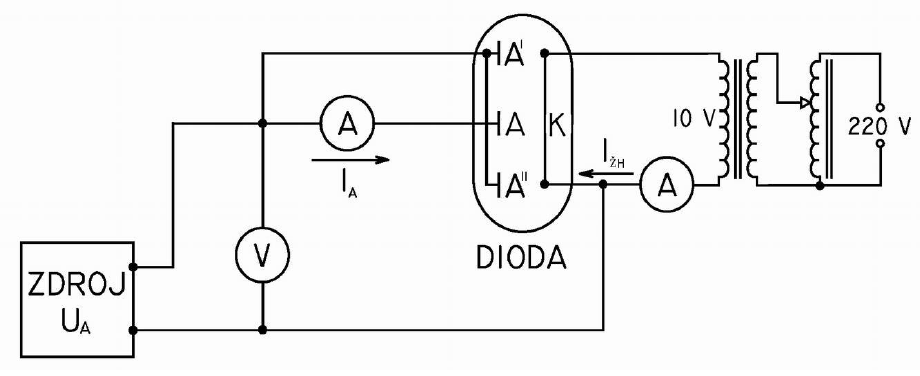
\includegraphics[width=12cm]{att/pyromet2.png}
			\caption{Zapojení pro měření náběhového proudu. Převzato z \cite{bib:zadani}.}
			\label{fig:s_aparatura_nasyc}
			\end{figure}	
			
			\begin{figure}[h!]
			\centering
			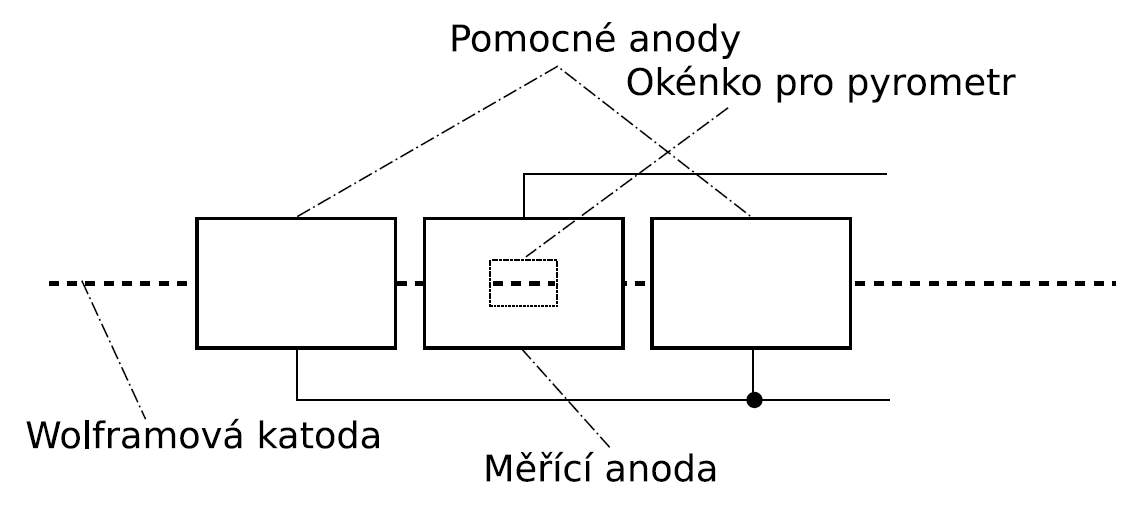
\includegraphics[width=10cm]{att/pyromet.png}
			\caption{Geometrie uspořádání vakuové diody s pomocnými anodami pro dosažení homogenního pole. \newline Převzato z \cite{bib:zadani}.}
			\label{fig:s_dida}
			\end{figure}
	
\clearpage
\section{Tabulky a grafy}
%%
	\begin{figure}[h!]
	\begin{center}
	    \vspace*{-1cm}
		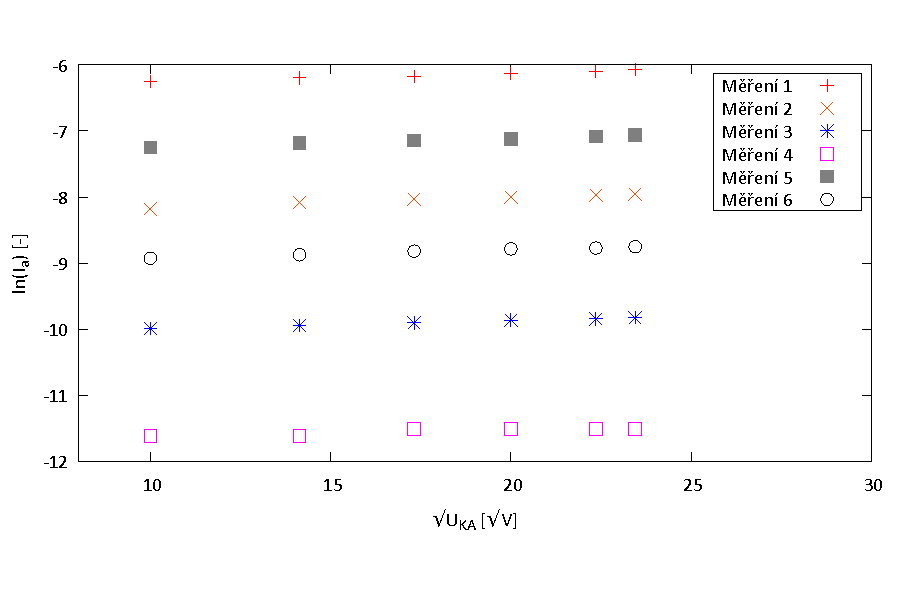
\includegraphics[width=\linewidth]{../gnuplot/termise.pdf}
	    \vspace*{-2cm}
		\caption{Měření nasyceného proudu; závislost celkového proudu $I_a$ (resp. jeho logaritmu) na napětí mezi katodou a anodou $U_{KA}$ (resp. jeho odmocnině).} 
		\label{fig:g_termise}
	\end{center}
	\end{figure}		

	\begin{figure}[h!]
	\begin{center}
	    \vspace*{-1cm}
		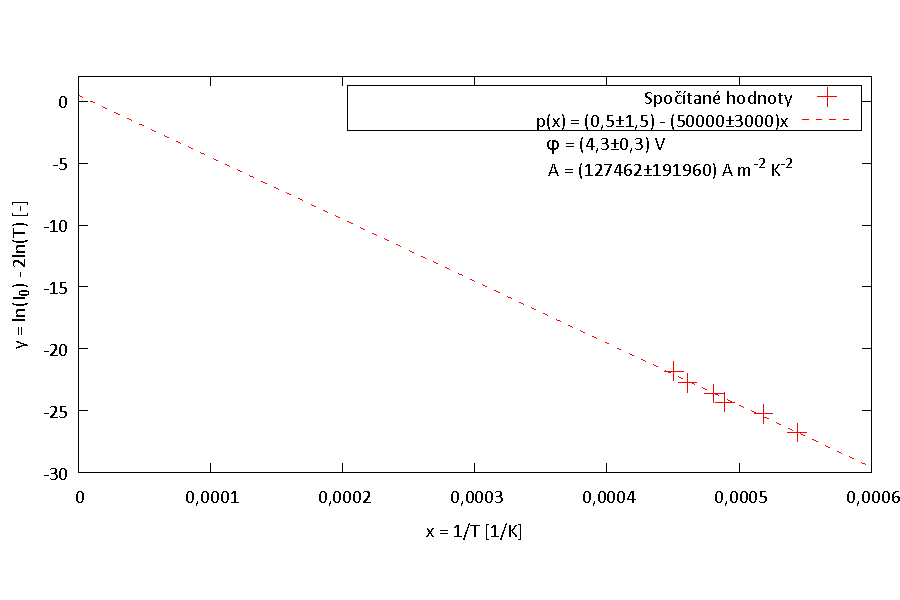
\includegraphics[width=\linewidth]{../gnuplot/termiserich.pdf}
	    \vspace*{-2cm}
		\caption{Měření nasyceného proudu; hodnoty spočítané z fitů každého z šesti měření pomocí (\ref{eq:sqrt_fit}) a jejich proložením podle (\ref{eq:fit_richardson}) získaná Richardsonova přímka. Z jejích parametrů pak podle (\ref{eq:phi_a_A}) spočítané $\varphi_v$ a $A$. } 
		\label{fig:g_termiserich}
	\end{center}
	\end{figure}		

	\begin{figure}[h!]
	\begin{center}
	    \vspace*{-1cm}
		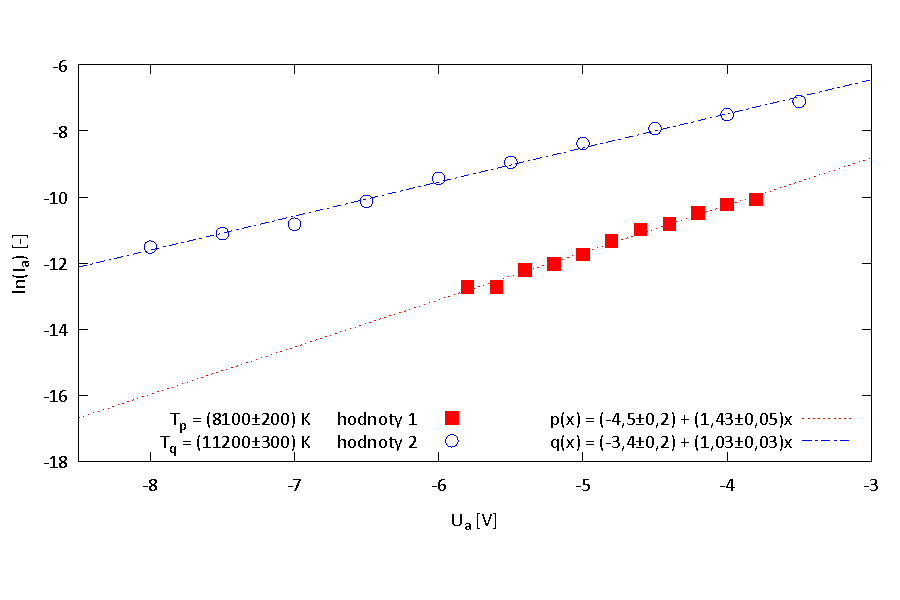
\includegraphics[width=\linewidth]{../gnuplot/nabeh.pdf}
	    \vspace*{-1,5cm}
		\caption{Měření náběhového proudu; závislost celkového proudu $I_a$ (resp. jeho logaritmu) na záporném napětí mezi katodou a anodou $U_{KA}$. Data jsou proložena fitem podle (\ref{eq:fit_nabeh}) a z něj jsou podle (\ref{eq:teplota_nabeh}) dopočítány teploty vlákna $T_p$ a $T_q$. } 
		\label{fig:g_nabeh}
	\end{center}
	\end{figure}		
	
	\begin{figure}[h!]
	\begin{center}
	    \vspace*{-1cm}
		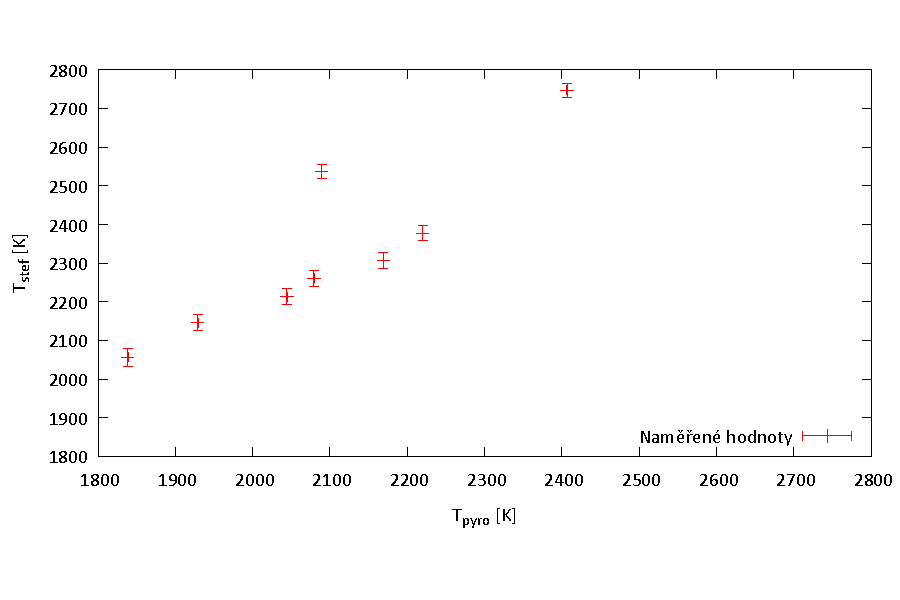
\includegraphics[width=\linewidth]{../gnuplot/stefpyro.pdf}
	    \vspace*{-1,5cm}
		\caption{Měření teploty pomocí Stefan-Boltzmannova zákona; závislost $T_{stef}$ spočítané podle (\ref{eq:stefan}) na teplotě určené pyrometrem $T_{pyro}$. } 
		\label{fig:g_stefpyro}
	\end{center}
	\end{figure}		
				
%\clearpage
% --- Konec dokumentu --------------------------------------------------


\end{document}

